\chapter{Evaluation}
\label{chapter:avaliacao}

This chapter presents the formal experimental campaign, bounded to ten days, run on the same server for G-FShield, both monoliths, and an all-features baseline. The single source for this analysis is the result set identified by the manifest whose SHA-256 is:
\begin{center}
\small\texttt{29fdc973ad6b243b297e34fcd539f5826aac4ce8a0870e8a5cea5caacfc9adc4}.
\end{center}
The historical CSV files in \texttt{tmp\_metrics/}, which contained the discrepancy between 25,873 raw lines and 25,836 lines with valid F1, are not combined with the new campaign. Neither count is therefore used as a comparative result.

\section{Experimental Protocol}

The preserved ERENO corpus contains 199,998 instances, 51 predictors, and nine classes. A stratified split, frozen before the searches with seed 20260825, produced 119,998 training, 40,000 validation, and 40,000 test instances. The SHA-256 prefixes for the source, training, validation, and test data are \texttt{60ebfcdc9c20}, \texttt{5876bf5570b7}, \texttt{c44a00ca554c}, and \texttt{05d393c5881a}; the full values are in the manifest. The test set remained unavailable to the search and was evaluated once after validation selected the solution.

Every final solution was reevaluated by the same image with Weka J48 3.8.6, a pruned tree, confidence factor 0.25, and a minimum of two instances per leaf. The primary metric is macro-F1 on the 0--1 scale; macro precision and recall, weighted F1, accuracy, and per-class F1 were preserved as complementary measures.

The matrix has 27 arms: 24 distributed configurations, two monoliths, and the baseline. Each arm uses independent seeds 42--49, totaling 216 valid runs. Distributed configurations cross four RCL rankings (IG, GR, SU, and ReliefF), two controllers (VND and RVND), and three initial local-search preferences (BF, IWSS, and IWSSR). All three operators remain enabled in each controller's portfolio. ReliefF uses 1,000 reference instances selected reproducibly from training with the run seed; classifier training, validation, and testing use the full splits.

Each algorithmic run received at most 3,000 s, including a 300-s reserve for shutdown and final evaluation. Search could also stop after 500 accepted improvements, with a minimum improvement of 0.0001. G-FShield uses cutoff 30, an initial solution of five features, and 100 iterations per operator. Monolith~1 runs GR followed by Bit-Flip, with cutoff 30, five features, and 100 local iterations. Monolith~2 runs GR followed by IWSS under VND, with the same cutoff and initial size and 100 local iterations. The baseline only trains and evaluates J48 with all 51 predictors. In every case, training fits the model, validation selects the best solution, and testing provides the common final measure.

All arms were confined to logical processors 8--15 on NUMA node~1, with an aggregate ceiling of eight CPUs and 16~GiB. Containers were sampled every 30 s with \texttt{docker stats}; CPU is summed in cores and memory is summed across containers belonging to the run. Other containers present on the host were recorded separately and are excluded from these sums. The campaign started on August 25, 2026 at 08:32 UTC and finished on September 1, 2026 at 03:36 UTC, before the ten-day limit, with no supervisor restart.

Twelve distributed attempts ended without a complete solution (\path{NO_COMPLETE_SOLUTION}) and were rejected by the artifact contract. The orchestrator reran only missing seed--arm combinations until each arm had eight valid results. There were consequently 228 attempts and 216 valid runs. All 208 search runs stopped at the time limit; the eight baseline runs exited normally.

In this chapter, a \emph{run} is one valid, independent replicate of an arm and seed. A \emph{final solution} is the subset selected on validation and evaluated once on test. An \emph{internal record} is a candidate row or event generated within that run; internal records are correlated and are not treated as replicates or end-to-end solutions.

\section{Predictive Quality and Dimensionality Reduction}

Table~\ref{tab:resultados-formais} summarizes the G-FShield configuration selected by the highest median validation macro-F1, both monoliths, and the baseline. Each arm uses eight runs. RF--VND--IWSSR obtained median test macro-F1 0.9448, interquartile range 0.9441--0.9449, 11 features, and 78.4\% reduction. The all-features baseline obtained 0.9378. The paired median difference was 0.0069 in favor of the selected configuration; this is a descriptive result, not demonstrated statistical superiority.

\begin{landscape}
\begin{table}[p]
\centering
\scriptsize
\caption{Final held-out test results and observed resources (medians of eight runs).}
\label{tab:resultados-formais}
\resizebox{.96\linewidth}{!}{%
\begin{tabular}{lrrrrrrrrrr}
\toprule
\textbf{Arm} & \textbf{Macro-F1} & \textbf{Precision} & \textbf{Recall} & \textbf{Accuracy} & \textbf{$|S|$} & \textbf{Reduction (\%)} & \textbf{Time (s)} & \textbf{CPU (cores)} & \textbf{Median RAM (MiB)} & \textbf{Peak RAM (MiB)} \\
\midrule
RF--VND--IWSSR & 0.9448 & 0.9463 & 0.9432 & 0.9343 & 11 & 78.4 & 2,815.3 & 2.104 & 4,726.0 & 5,858.3 \\
Monolith 1 (GR--BF) & 0.9397 & 0.9399 & 0.9396 & 0.9293 & 5 & 90.2 & 2,712.5 & 1.069 & 1,531.4 & 1,959.4 \\
Monolith 2 (GR--IWSS) & 0.8411 & 0.8571 & 0.8454 & 0.8412 & 5 & 90.2 & 2,725.9 & 1.003 & 1,394.7 & 1,788.9 \\
All 51 features & 0.9378 & 0.9402 & 0.9358 & 0.9272 & 51 & 0.0 & 72.5 & 1.044 & 748.4 & 820.0 \\
\bottomrule
\end{tabular}}

\vspace{0.4em}
\parbox{.96\linewidth}{\footnotesize F1, precision, and recall are macro averages. CPU is the temporal median of the sum across run containers and then the median across seeds. Median and peak RAM use the same boundary. Time is end-to-end, including startup, search, validation selection, controlled shutdown, and final evaluation.}
\end{table}
\end{landscape}

Monolith~1 obtained median F1 0.9397; Monolith~2 had median 0.8411 and high dispersion (mean 0.7343; standard deviation 0.2013). The baseline is deterministic under the adopted setup and repeated 0.9378 for all eight seeds. Across the 24 distributed configurations, median F1 ranged from 0.8671 to 0.9448; the median across configurations was 0.9418. Every configuration produced eight distinct final subsets. Median subset size ranged from 5 to 17 features, corresponding to reductions from 90.2\% to 66.7\%.

\begin{figure}[p]
  \centering
  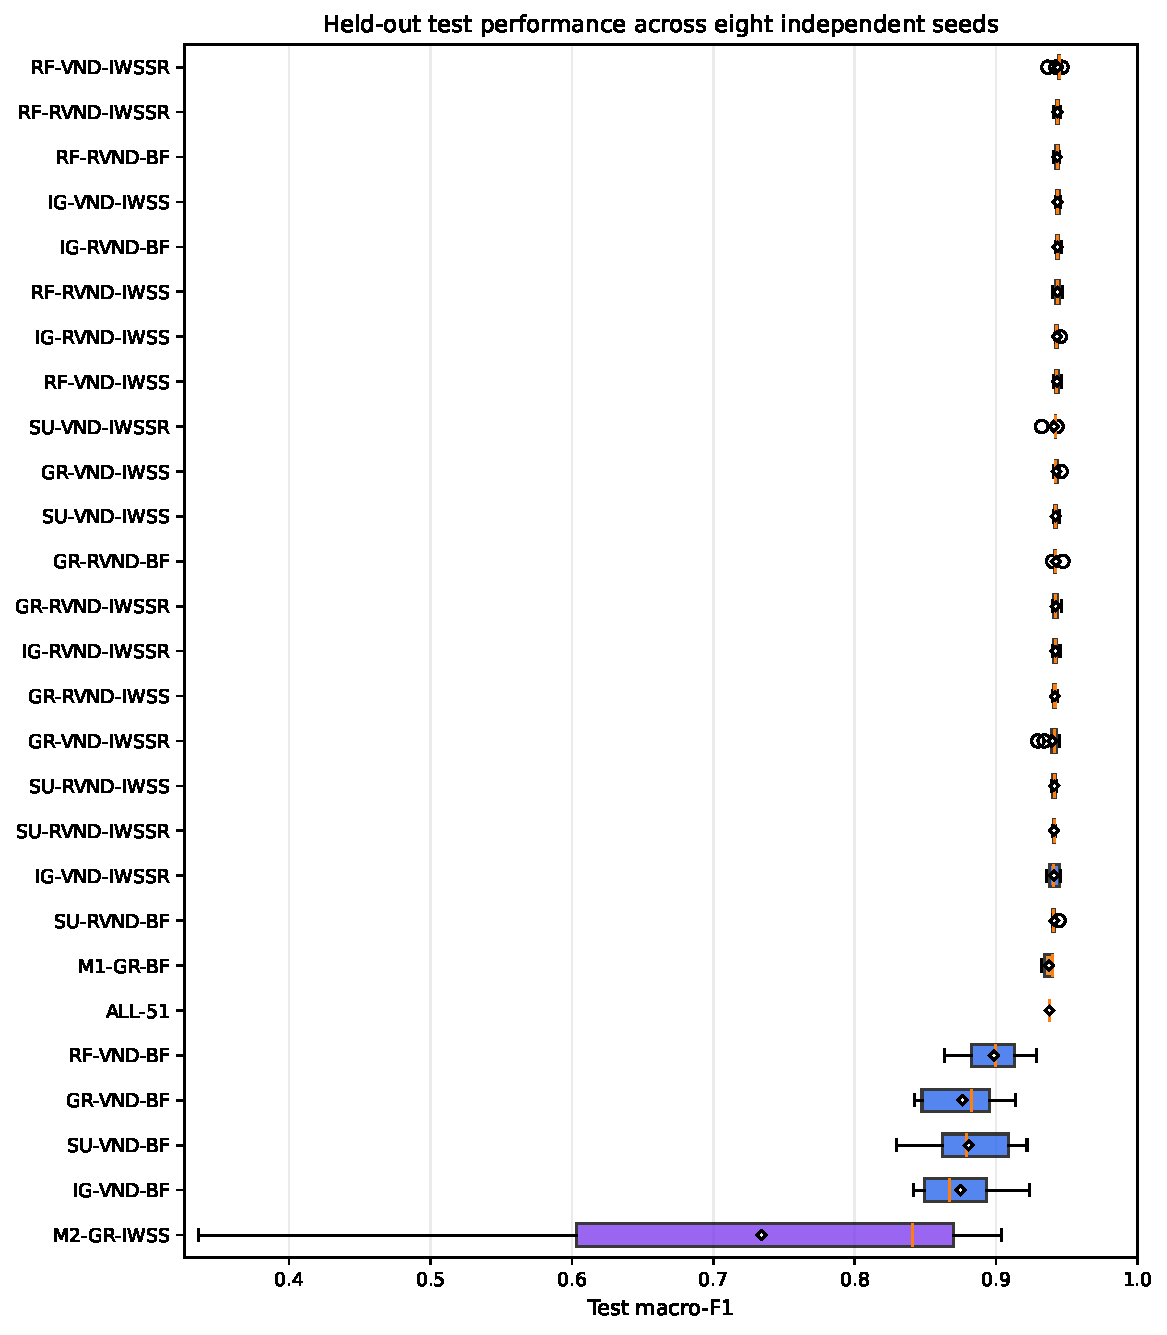
\includegraphics[width=.94\linewidth,height=.80\textheight,keepaspectratio]{fig/gfshield/campaign-test-f1.pdf}
  \caption{Test macro-F1 distributions for all 27 arms and eight seeds per arm.}
  \label{fig:campaign-test-f1}
\end{figure}

\begin{landscape}
\begin{figure}[p]
  \centering
  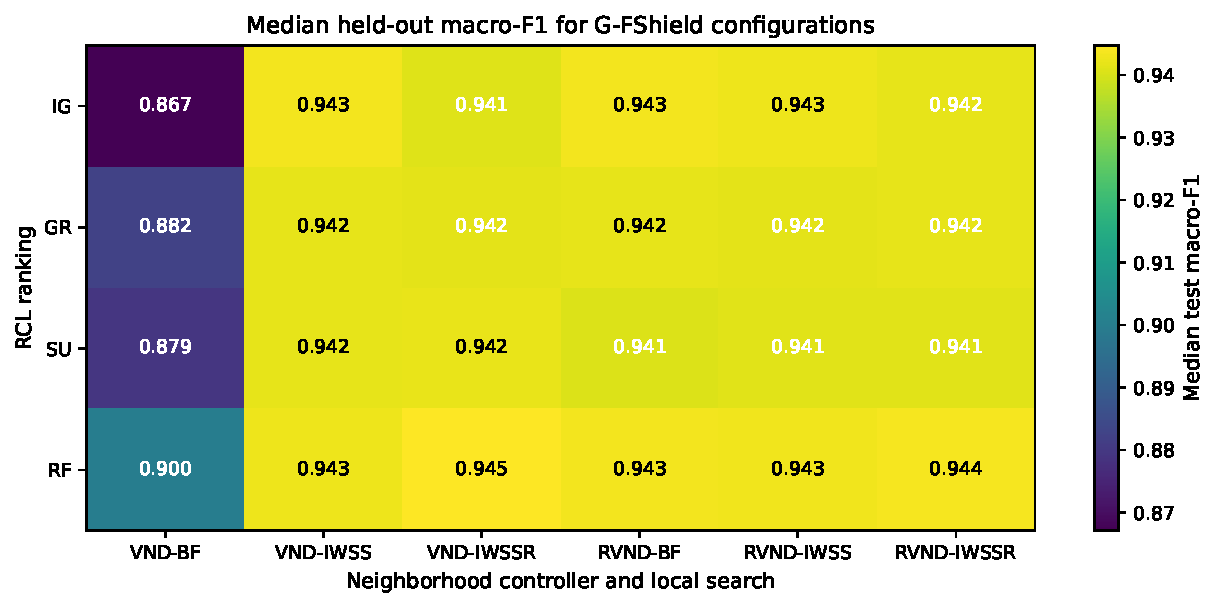
\includegraphics[width=.96\linewidth,height=.80\textheight,keepaspectratio]{fig/gfshield/campaign-configuration-heatmap.pdf}
  \caption{Median test macro-F1 for the 24 distributed configurations.}
  \label{fig:campaign-heatmap}
\end{figure}
\end{landscape}

Figure~\ref{fig:campaign-heatmap} shows that the four VND--BF combinations remained below configurations that effectively explored IWSS/IWSSR. This outcome depends on the protocol and the implemented search objective; it does not establish that an operator is universally inferior. Figure~\ref{fig:campaign-quality-reduction} presents the quality--reduction relationship. RF--VND--IWSSR descriptively exceeds the baseline's F1 with 40 fewer features, while Monolith~1 uses only five features and preserves F1 close to the baseline.

\begin{landscape}
\begin{figure}[p]
  \centering
  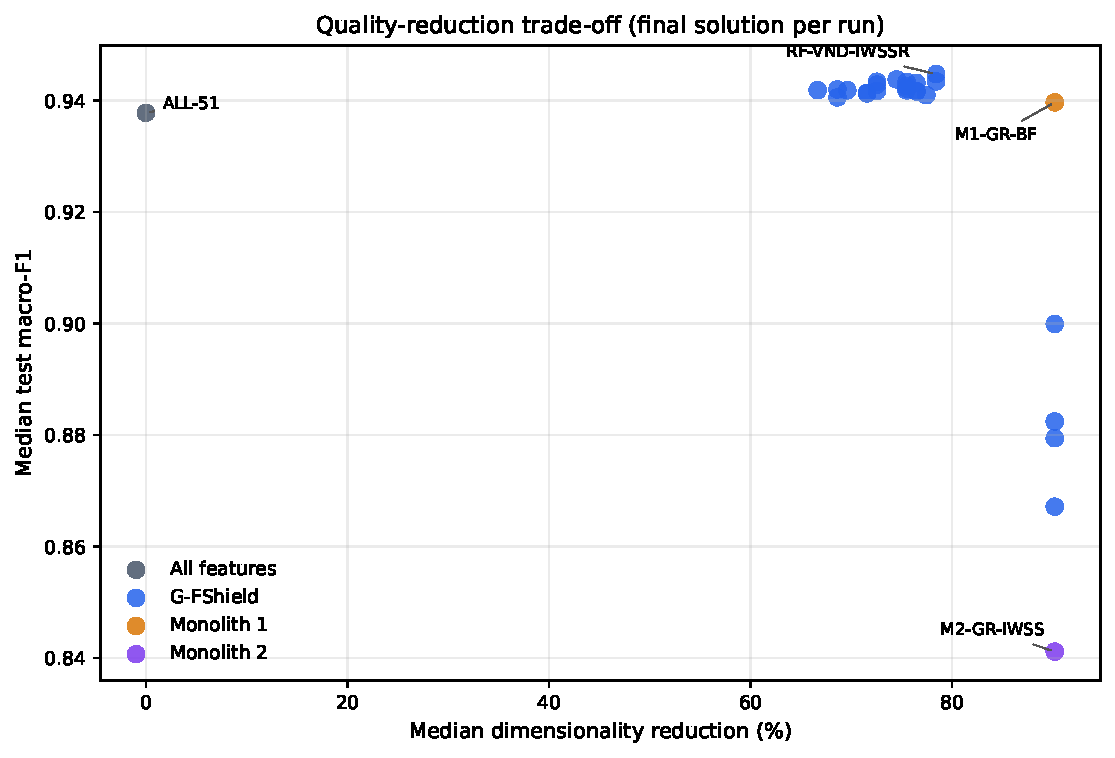
\includegraphics[width=.96\linewidth,height=.80\textheight,keepaspectratio]{fig/gfshield/campaign-quality-reduction.pdf}
  \caption{Trade-off between median macro-F1 and dimensionality reduction of final solutions.}
  \label{fig:campaign-quality-reduction}
\end{figure}
\end{landscape}

Per-class performance (Figure~\ref{fig:campaign-per-class}) exposes information hidden by the average: for RF--VND--IWSSR, median F1 is 0.7179 for \textit{grayhole}, 0.8451 for \textit{normal}, and at least 0.9565 for the other seven classes. Macro-F1 close to 0.945 therefore does not imply uniform performance across attacks.

\begin{landscape}
\begin{figure}[p]
  \centering
  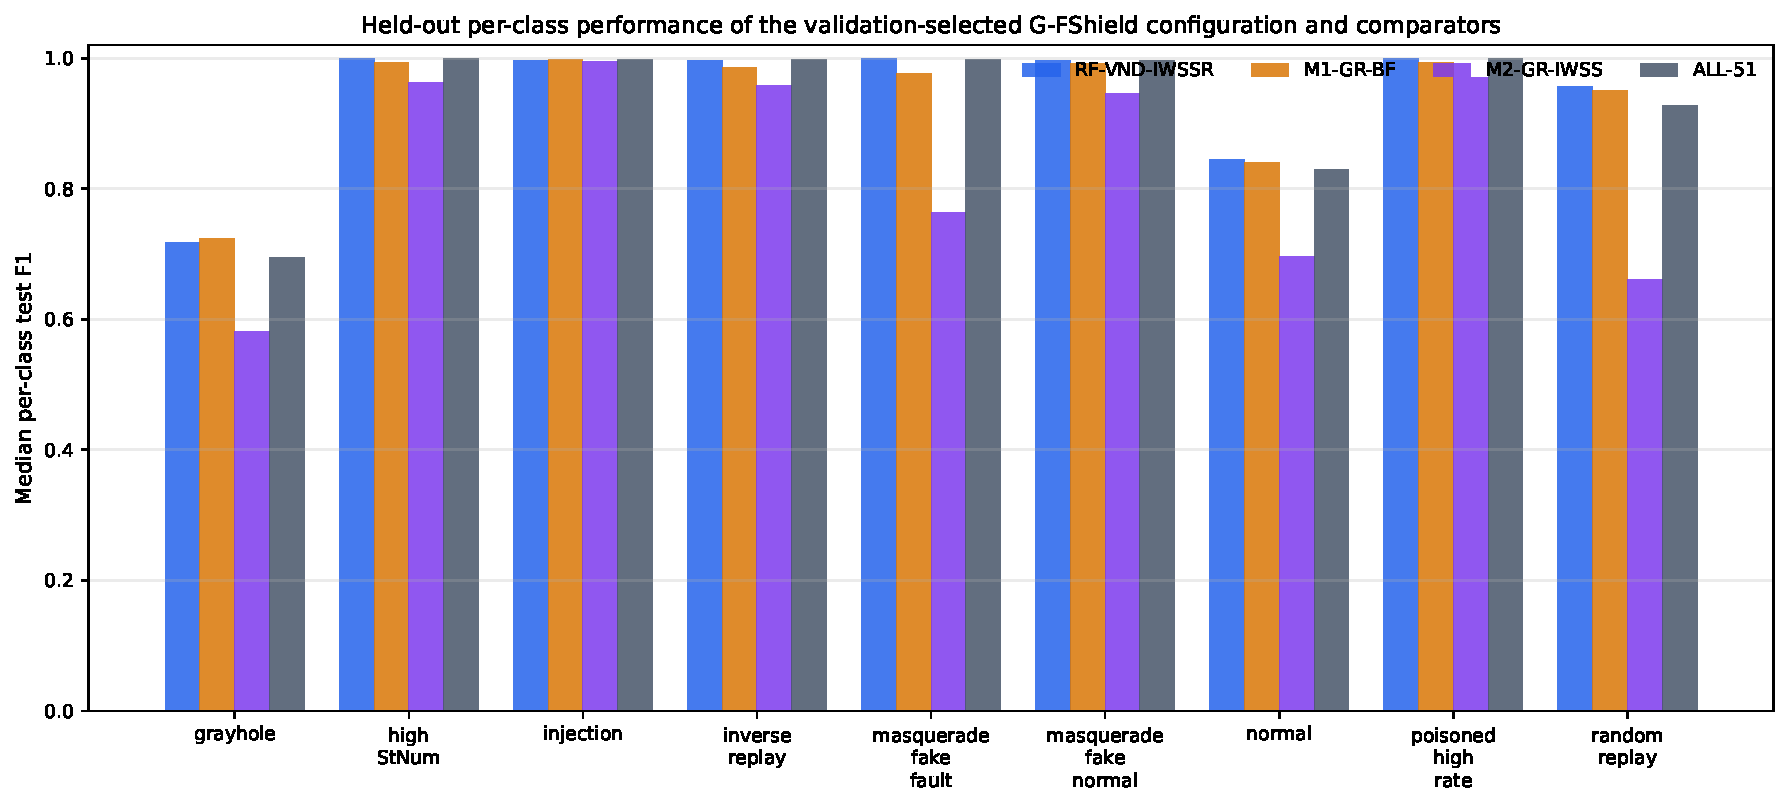
\includegraphics[width=.97\linewidth,height=.80\textheight,keepaspectratio]{fig/gfshield/campaign-per-class-f1.pdf}
  \caption{Median per-class test F1 for the validation-selected distributed configuration and comparators.}
  \label{fig:campaign-per-class}
\end{figure}
\end{landscape}

\section{Time, Resources, and Statistical Interpretation}

Because all 208 searches stopped at the same limit, median end-to-end time ranged from 2,706 to 2,847 s by configuration. These values do not demonstrate faster convergence. None of the 24 distributed configurations reached internal F1 $\geq 0.95$. Audit of the image-source commit confirmed that this internal score was already multiclass macro-F1; the binary routine containing \texttt{normalClass=0} was disabled. Nevertheless, the campaign did not preserve an equivalent cumulative timeline for every candidate in both monoliths: their CSV files record individual evaluation duration rather than elapsed time since run start. A valid time-to-threshold comparison therefore cannot be computed from this campaign. That outcome requires comparable monotonic timestamps in both arms, validation-only evaluation, and censoring at the same deadline.

Under the same aggregate ceiling, distributed runs used a global median of 3.56 cores and median peak of 5.45, compared with approximately 1.07/1.83 for Monolith~1 and 1.00/1.82 for Monolith~2. Distributed memory had a global median of 5,317~MiB and median peak of 6,757~MiB, compared with median peaks of 1,959 and 1,789~MiB for the monoliths. This quantifies observed consumption but does not prove efficiency: the distributed pipeline aggregates multiple Java processes and messaging infrastructure, while the compared arms execute different rankings and local-search operators.

\begin{landscape}
\begin{figure}[p]
  \centering
  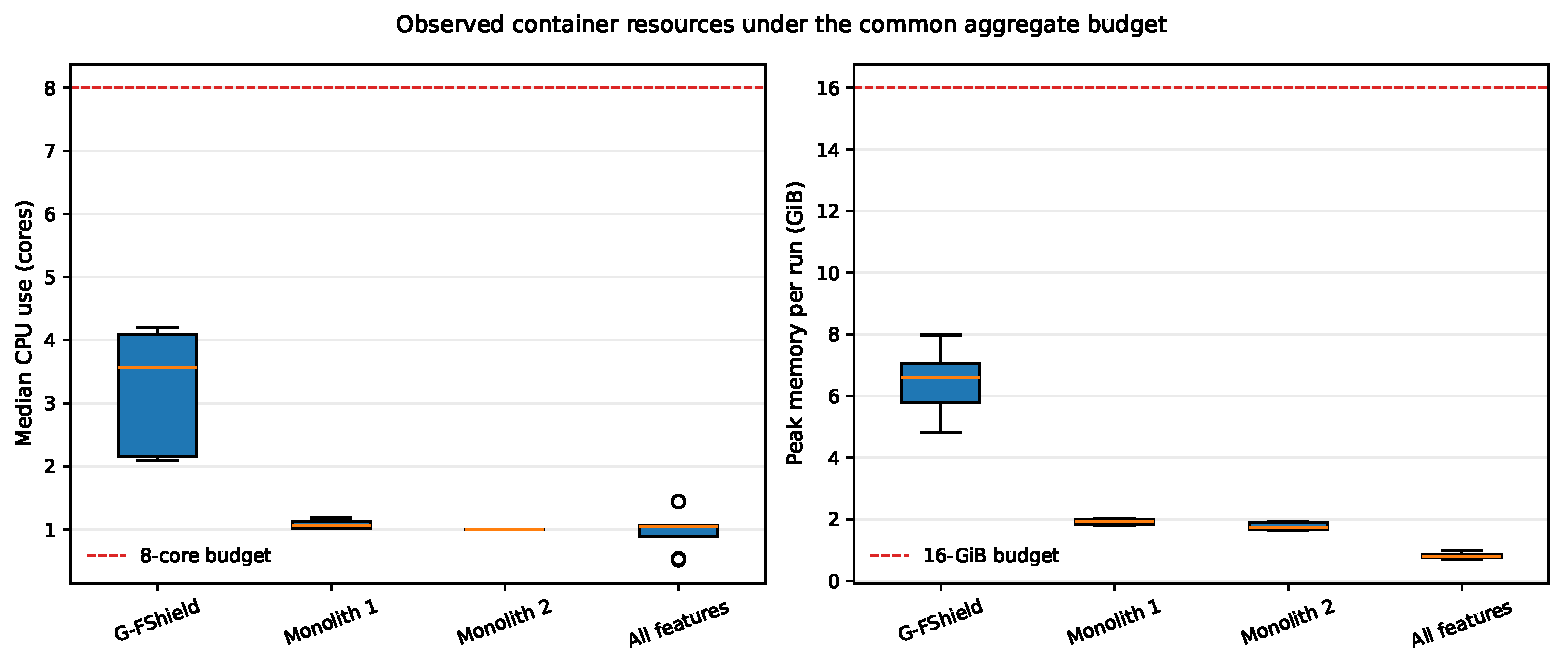
\includegraphics[width=.96\linewidth,height=.80\textheight,keepaspectratio]{fig/gfshield/campaign-resources.pdf}
  \caption{Observed CPU and memory by architecture under the common aggregate ceiling of eight CPUs and 16~GiB.}
  \label{fig:campaign-resources}
\end{figure}
\end{landscape}

As an exploratory analysis, each distributed configuration was paired by seed with each comparator using a two-sided exact sign-flip test and paired rank-biserial effect size. Holm correction was applied separately to each comparator's family of 24 tests. RF--VND--IWSSR recorded seven wins and one loss against the baseline and eight wins against each monolith; all three adjusted $p$-values were 0.1875. None of the 72 adjusted comparisons was below 0.05. With eight seeds, intervals and tests have low power; the results support descriptive differences, not claims of significance or architectural causality.

\section{Paired Causal Architecture Experiment}
\label{sec:architecture-causal}

To separate architecture from algorithm, a second campaign compared two implementations of the same RF--VND--IWSSR sequence: the G-FShield pipeline and a sequential monolithic executable. Operator specification, Weka J48, objective function, data splits, parameters, seeds, the 2,700-s selection deadline, and the aggregate ceiling of six CPUs and 12~GiB were fixed. The distributed arm used three consumers so that one construction could progress while another solution underwent local search; the monolith executed the same stages sequentially. AB/BA order was balanced across seeds 42--71. Because the implementations use different runtimes, residual implementation effects cannot be completely excluded.

The protocol prespecified censored time to validation macro-F1 $\geq 0.94$ as the primary outcome, defining the paired difference as distributed minus monolith and applying a one-sided permutation test. A favorable interpretation also required the one-sided 95\% lower bound of the mean held-out macro-F1 difference to be no lower than $-0.005$. Candidates were scored only on validation; held-out test was queried once for the final solution. The campaign completed 60 valid runs, or 30 pairs. Seven earlier distributed attempts failed during Kafka/ZooKeeper startup and were rejected and retried by the artifact contract; none of the 60 valid manifests had a checksum error.

\begin{landscape}
\begin{table}[p]
\centering
\scriptsize
\caption{Causal campaign: architecture medians and paired comparisons across 30 seeds.}
\label{tab:architecture-causal}
\resizebox{.96\linewidth}{!}{%
\begin{tabular}{lrrrl}
\toprule
\textbf{Measure} & \textbf{G-FShield} & \textbf{Monolith} & \textbf{Paired median difference} & \textbf{Result} \\
\midrule
Test macro-F1 & 0.945529 & 0.944699 & $+0.000017$ & 15 wins, 10 ties, 5 losses \\
Time to F1 $\geq 0.94$ (s) & 940.077 & 701.255 & $+422.740$ & $p=0.000795$; distributed slower \\
Normalized anytime AUC & 0.879884 & 0.897069 & $-0.016898$ & $p_{Holm}=0.000055$ \\
Candidates per second & 0.1074 & 0.0739 & $+0.0317$ & 30/30 pairs; $p_{Holm}=0.000055$ \\
Median utilized CPU (cores) & 4.076 & 1.004 & $+3.070$ & 30/30 pairs \\
CPU-h per candidate & 0.010875 & 0.003821 & $+0.007095$ & 0/30 pairs favorable to distributed \\
GiB-h per candidate & 0.012366 & 0.004904 & $+0.007397$ & 0/30 pairs favorable to distributed \\
Construction--local-search overlap & 99.998\% & 0\% & $+99.998$ pp & 30/30 pairs; $p_{Holm}=0.000055$ \\
Dimensionality reduction & 78.43\% & 76.47\% & $+1.96$ pp & 18 wins, 12 ties; $p_{Holm}=0.000080$ \\
\bottomrule
\end{tabular}}
\end{table}
\end{landscape}

The primary outcome contradicts the hypothesis of lower latency for a single request: G-FShield took longer to reach 0.94 in 23 of 30 pairs. The paired mean test macro-F1 difference was $-0.001759$, and its one-sided 95\% lower bound was $-0.005615$; because it narrowly crossed the prespecified negative margin of $-0.005$, the noninferiority guardrail was not satisfied either. The 0.95 threshold was censored in every pair and does not distinguish the architectures.

Conversely, decomposition produced the intended architectural mechanism: almost all local search occurred concurrently with construction, whereas monolithic execution remained sequential. This increased median candidate-evaluation throughput by approximately 45\%, but required roughly four times as much simultaneous CPU and incurred higher CPU and memory cost per candidate. Figure~\ref{fig:architecture-speed-processing} presents these effects together. Thus, ``better'' depends on the objective: G-FShield is superior in observable parallelism, raw throughput, and, under this protocol, dimensionality reduction; the monolith is superior in latency to 0.94 and resource efficiency. Global superiority of the distributed architecture was not demonstrated.

\begin{landscape}
\begin{figure}[p]
  \centering
  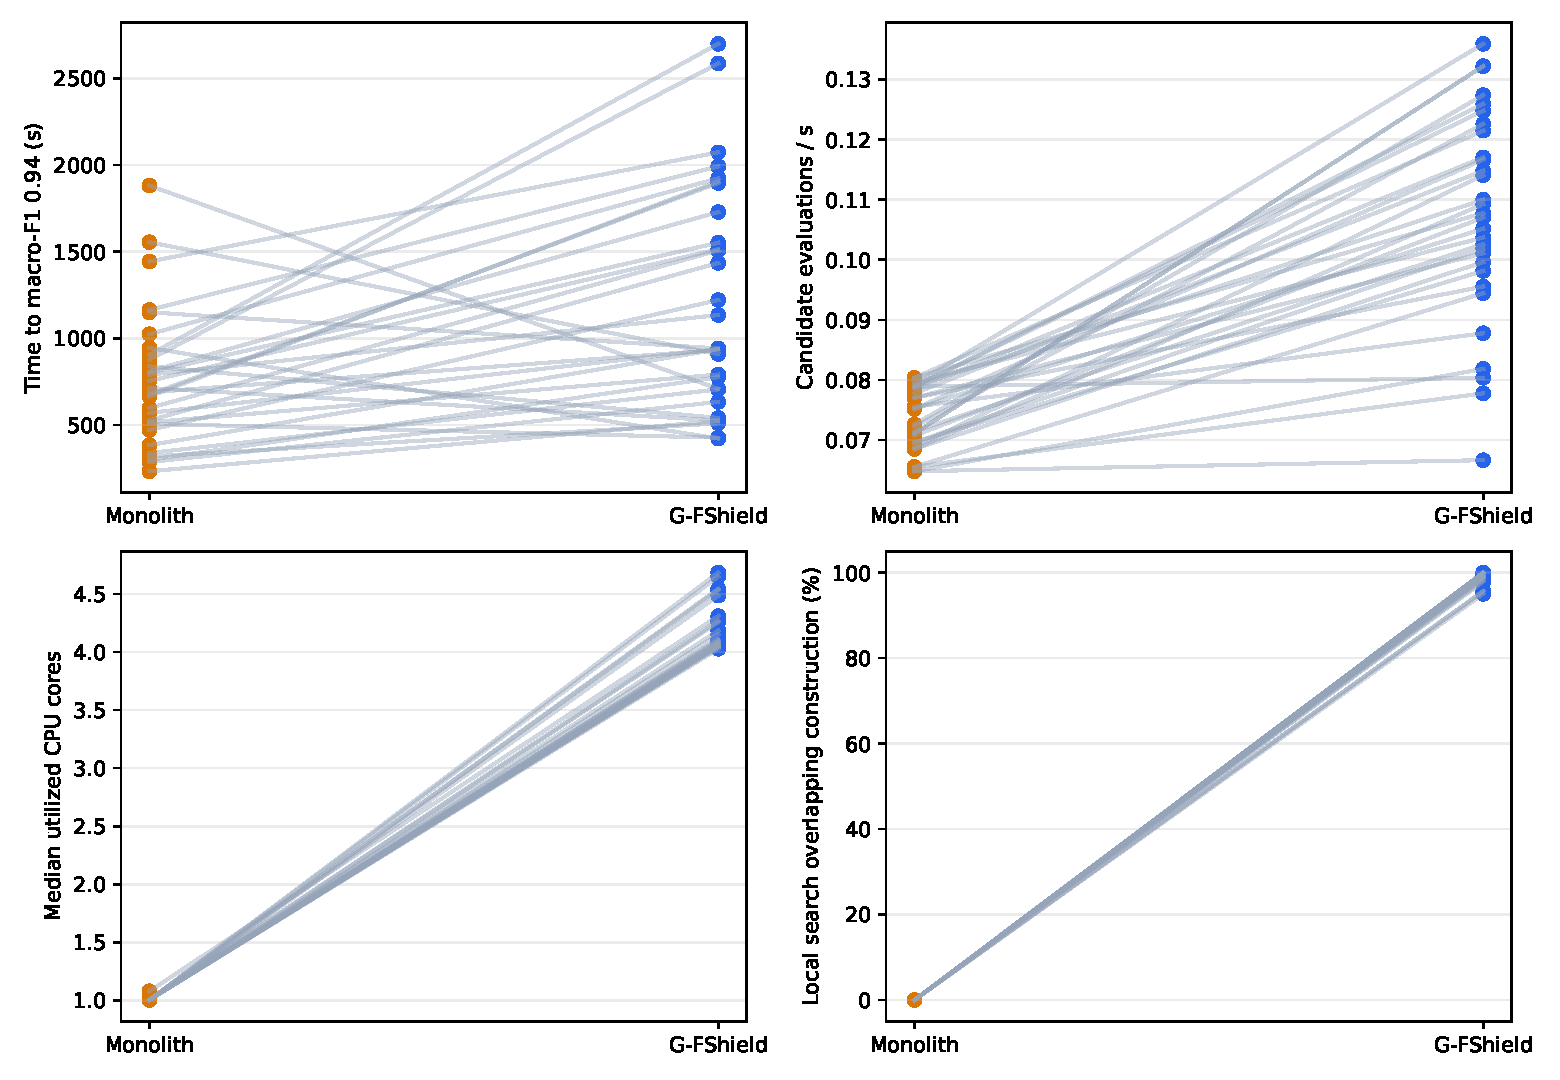
\includegraphics[width=.96\linewidth,height=.80\textheight,keepaspectratio]{fig/gfshield/architecture-speed-processing.pdf}
  \caption{Paired comparisons of time to macro-F1 0.94, candidate throughput, utilized CPU, and overlap between construction and local search.}
  \label{fig:architecture-speed-processing}
\end{figure}
\end{landscape}

The median best-validation trajectory (Figure~\ref{fig:architecture-anytime}) explains the result: the monolith reaches good solutions early, whereas greater distributed throughput does not automatically translate into quality progress. Post-hoc inspection suggested counting \emph{distinct} subsets with validation F1 $\geq 0.945$ by the deadline as a high-quality-solution yield measure. Because this threshold was selected after observing these data, it is not used as confirmation in this campaign; it was frozen for a new independent campaign with seeds 72--101.

\begin{landscape}
\begin{figure}[p]
  \centering
  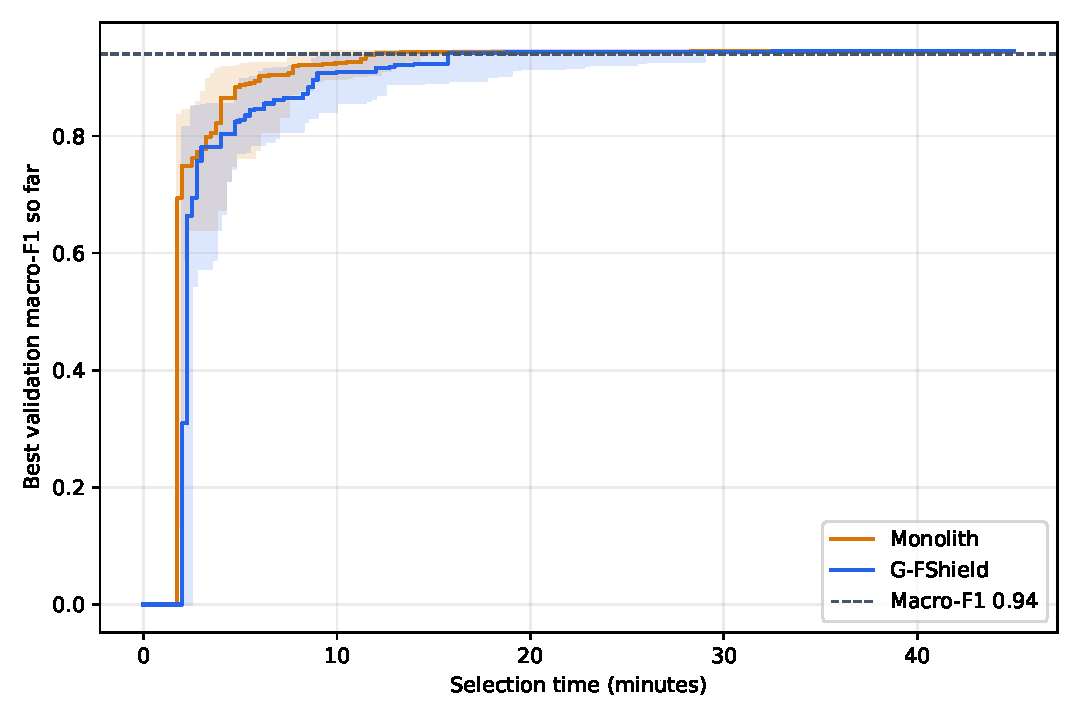
\includegraphics[width=.96\linewidth,height=.80\textheight,keepaspectratio]{fig/gfshield/architecture-anytime-validation-f1.pdf}
  \caption{Median best-validation trajectory during the 45-minute selection period. Bands show the interquartile range across seeds.}
  \label{fig:architecture-anytime}
\end{figure}
\end{landscape}

\section{Observability and Traceability}

Each run preserves \texttt{campaign\_id}, \texttt{run\_id}, arm, seed, parameters, data hashes, resolved command, states, stop reason, UTC and monotonic timestamps, selected solution, final metrics, best-solution messages, internal CSV files, logs, and container telemetry. A checksum manifest for every run detects artifact changes, and campaign state reconstructs attempts, rejections, and retries.

In the application, the backend persists events for initial solution, neighborhood restart, search progress, refined solution, and best solution, plus topic, partition, offset, state, \texttt{seedId}, timestamps, and JSON content when available. The formal campaign adds \texttt{campaign\_id}, \texttt{run\_id}, and \texttt{request\_id} to its experimental flows, removing ambiguity among concurrent runs within this protocol. Event completeness, instrumentation overhead, loss/duplication under failure, recovery time, and reprocessing success were not measured. Fault tolerance and resilience therefore remain design objectives.

\section{Threats to Validity}

\textbf{Internal validity.} In the first campaign, CPU, memory, CPU set, data, seeds, time limit, J48, and macro-F1 were controlled, but the comparators executed different algorithmic sequences. The subsequent causal experiment removed this confounding, recorded equivalent cumulative trajectories, and balanced AB/BA order. Possible shared-host interference and startup effects remain: 12 attempts in the first campaign and seven distributed attempts in the causal campaign were rejected and retried because they did not produce a complete artifact. This preserves the seed matrix but conditions analysis on runs that initialized correctly.

\textbf{Construct validity.} The primary measure is macro-F1 on held-out test data, and runs, final solutions, and internal records are separated. The median per arm reduces the influence of extremes but does not summarize the full distribution. CPU and memory measure containers, not energy or monetary cost. The 0.95 threshold is an analytical convention, not an operational requirement.

\textbf{Conclusion validity.} In the first campaign, eight seeds provide low power, the baseline is deterministic, and choosing among 24 configurations introduces multiple selection. In the causal experiment, the 30 pairs, primary outcome, and quality guardrail were defined before analysis; internal candidates were not treated as replicates. Secondary measures use Holm correction. The high-quality-subset count proposed after analysis is explicitly exploratory and requires confirmation on independent seeds 72--101.

\textbf{External validity.} Evidence covers one server, one IEC~61850 corpus, one split, and J48. It does not demonstrate generalization to other corpora, classifiers, concurrent loads, replica counts, hardware, failures, or continuous ingestion. Future work should repeat the protocol on multiple datasets and evaluate scaling and recovery separately.
